% System architecture. Build: pdflatex architecture.tex  ->  architecture.pdf (\includegraphics it in the thesis).
% Translate the labels for the Vietnamese version.
\documentclass[tikz,border=6pt]{standalone}
\usepackage[T1]{fontenc}
\usepackage{helvet}
\renewcommand{\familydefault}{\sfdefault}
\usetikzlibrary{arrows.meta,fit,backgrounds}
\definecolor{ink}{HTML}{0B0B0B}
\definecolor{ink2}{HTML}{52514E}
\definecolor{line}{HTML}{8A8984}
\definecolor{wash}{HTML}{EEF4FC}
\definecolor{blue}{HTML}{2A78D6}
\begin{document}
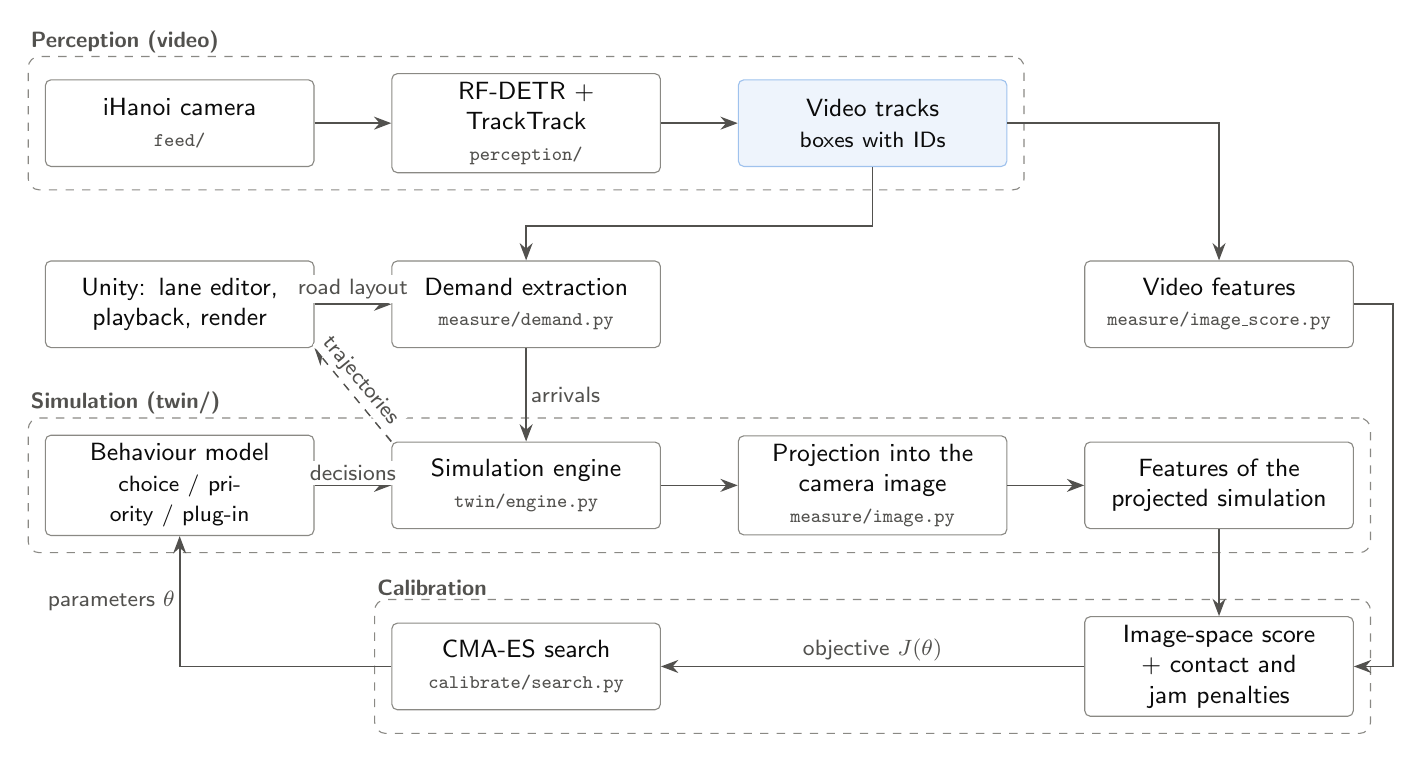
\begin{tikzpicture}[
    font=\small, >={Stealth[length=2.2mm]},
    box/.style={draw=line, rounded corners=2pt, fill=white, align=center, inner sep=3pt, minimum height=11mm,
                text width=32mm, text=ink},
    data/.style={box, fill=wash, draw=blue!45},
    path/.style={font=\scriptsize\ttfamily, text=ink2},
    group/.style={draw=line, dashed, rounded corners=4pt, inner sep=6pt},
    lbl/.style={font=\footnotesize\bfseries, text=ink2, anchor=south west, inner sep=1pt},
    tag/.style={font=\footnotesize, text=ink2, fill=white, inner sep=1.5pt},
    arr/.style={->, draw=ink2, line width=0.6pt}]

  % Columns 0, 4.4, 8.8, 13.2 cm; rows 0, -2.3, -4.6, -6.9 cm.
  \node[box]  (cam)    at (0, 0)      {iHanoi camera\\ \textcolor{ink2}{\scriptsize\ttfamily feed/}};
  \node[box]  (det)    at (4.4, 0)    {RF-DETR + TrackTrack\\ \textcolor{ink2}{\scriptsize\ttfamily perception/}};
  \node[data] (tracks) at (8.8, 0)    {Video tracks\\ \footnotesize boxes with IDs};

  \node[box]  (unity)  at (0, -2.3)   {Unity: lane editor,\\ playback, render};
  \node[box]  (demand) at (4.4, -2.3) {Demand extraction\\ \textcolor{ink2}{\scriptsize\ttfamily measure/demand.py}};
  \node[box]  (vfeat)  at (13.2, -2.3){Video features\\ \textcolor{ink2}{\scriptsize\ttfamily measure/image\_score.py}};

  \node[box]  (model)  at (0, -4.6)   {Behaviour model\\ \footnotesize choice / priority / plug-in};
  \node[box]  (engine) at (4.4, -4.6) {Simulation engine\\ \textcolor{ink2}{\scriptsize\ttfamily twin/engine.py}};
  \node[box]  (proj)   at (8.8, -4.6) {Projection into the\\ camera image\\ \textcolor{ink2}{\scriptsize\ttfamily measure/image.py}};
  \node[box]  (sfeat)  at (13.2, -4.6){Features of the\\ projected simulation};

  \node[box]  (cma)    at (4.4, -6.9) {CMA-ES search\\ \textcolor{ink2}{\scriptsize\ttfamily calibrate/search.py}};
  \node[box]  (score)  at (13.2, -6.9){Image-space score\\ + contact and jam penalties};

  \draw[arr] (cam) -- (det);
  \draw[arr] (det) -- (tracks);
  \draw[arr] (tracks.south) -- ++(0,-0.75) -| (demand.north);
  \draw[arr] (tracks.east) -| (vfeat.north);
  \draw[arr] (unity) -- node[tag, above] {road layout} (demand);
  \draw[arr] (demand) -- node[tag, right] {arrivals} (engine);
  \draw[arr] (model) -- node[tag, above] {decisions} (engine);
  \draw[arr] (engine) -- (proj);
  \draw[arr] (proj) -- (sfeat);
  \draw[arr] (sfeat) -- (score);
  \draw[arr] (vfeat.east) -- ++(0.5,0) |- (score.east);
  \draw[arr] (score) -- node[tag, above] {objective $J(\theta)$} (cma);
  \draw[arr] (cma.west) -| node[tag, pos=0.75, left] {parameters $\theta$} (model.south);
  \draw[arr, dashed] (engine.north west) -- node[tag, sloped, above, pos=0.55] {trajectories} (unity.south east);

  \begin{scope}[on background layer]
    \node[group, fit=(cam)(det)(tracks)] (g1) {};
    \node[lbl] at (g1.north west) {Perception (video)};
    \node[group, fit=(model)(engine)(proj)(sfeat)] (g2) {};
    \node[lbl] at (g2.north west) {Simulation (twin/)};
    \node[group, fit=(cma)(score)] (g3) {};
    \node[lbl] at (g3.north west) {Calibration};
  \end{scope}
\end{tikzpicture}
\end{document}
